In this section, we outline the methodologies employed.
Our approach encompasses synthetic dataset engineering,
a novel framework, loss function modifications and a comprehensive grasping pipeline.

Firstly, we focus on synthetic dataset engineering accommodating spatial, colour and background augmentation. The colour and
background augmentations help the framework to predict object-oriented descriptors.
Secondly, we present a novel framework designed to reduce computational resource consumption with loss function
modifications to optimize performance. Lastly, we introduce a comprehensive robot grasping pipeline exploiting the generalizing capabilities of our framework.

\subsection{Dataset Engineering}

We have chosen the cap object for creating a synthetic dataset as the cap mesh models are readily available in the Shapenet library~\cite{chang2015shapenet} as it contains rich object information, including textures.
Furthermore, we choose five cap models from the Shapenet library and use Blenderproc~\cite{blenderproc}
to generate the synthetic dataset. We save one RGB image, mask, and depth for each cap model from the synthetic scene.
Additionally, we employ synthetic augmentations as proposed in \cite{adrian2022efficient} to synthetically
spatial augment the cap's position and rotation in an image, including background randomization
using Torchvision~\cite{marcel2010torchvision} library. An augmented image pair is sampled randomly to generate camera poses for different viewpoints. Additionally, image-pair correspondences are computed
\footnote[1]{GitHub Link: \emph{link is made anonymous for the review}}
as illustrated in the Figure~\ref{fig:image_augs}. We only compute 24 image-pair correspondences
for an image-pair as we found that 24 image correspondences yield stable computation for translation and rotation for all the objects.
Using depth information,
we project the computed correspondences to the camera frame and compute the relative transformation between
two camera-frame coordinates of the correspondences using Kabsch's transformation~\cite{kabsch}.
Moreover, mask and depth images are not used during inference.

\begin{figure}[htb]
    \centering
    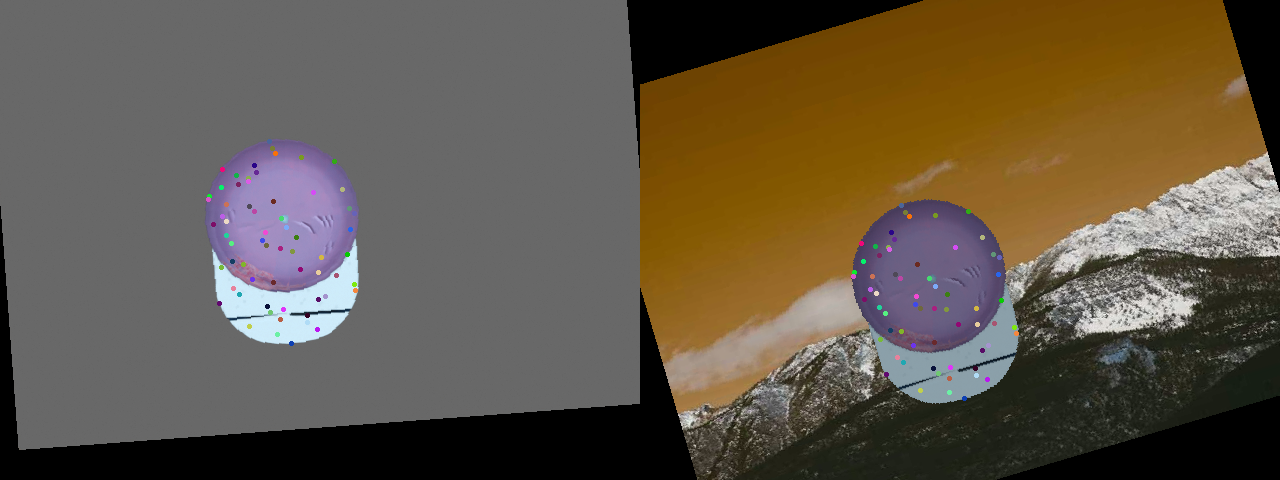
\includegraphics[scale=0.175]{images/debug_correspondences.png}
    \caption{Depiction of image synthetic spatial augmentation and correspondences mapping in an image-pair. The colored encoded dots in the figure represents correspondences in an image-pair.}
    \label{fig:image_augs}
\end{figure}


\subsection{Framework \& Mining Strategy}

As a backbone, we employ ResNet-34 architecture \cite{resnet}.
We preserve the last convolution layer and remove the pooling and linear layers. The backbone downsamples the RGB image $I_{RGB} \in \mathbb{R}^{H \times W \times 3}$
to dense features $I_d \in \mathbb{R}^{h \times w \times D}$
such that $ h \ll H, w \ll W \text{ and } D \in \mathbb{N}^+$.
We upsample the dense features from the identity layer
(being identical to the last convolution layer in the backbone) as illustrated in the Figure~\ref{fig:modified_dnn} in page~\pageref{fig:modified_dnn} as follows:
\begin{equation}
    f_U: I \in \mathbb{R}^{h \times w \times D} \rightarrow I_D \in \mathbb{R}^{H \times W \times D}.
\end{equation}
The upsampled dense features are extracted and treated as dense visual local descriptors produced from the DON. In otherwords
we extract or mine the representations from the backbone.
Similarly as in \cite{suwajanakorn2018discovery}, we stack spatial-probability regressing layer and
depth regressing layer on top of the identity layer to predict $N \in \mathbb{N}^+$ number of keypoint's spatial-probability as follows:
\begin{equation}
    f_S: I_d \in \mathbb{R}^{h \times w \times D} \rightarrow I_s^N \in \mathbb{R}^{h \times w \times N},
\end{equation}
and depth as follows:
\begin{equation}
    f_D: I_d \in \mathbb{R}^{h \times w \times D} \rightarrow I_{\hat{d}} \in \mathbb{R}^{h \times w \times N}.
\end{equation}

We incorporate continuous sampling method $f_E$ from \parencites{florence2020dense}{suwajanakorn2018discovery}
to convert the upsampled predicted spatial-probability and depth of a keypoint to spatial-depth expectation as follows:
\begin{equation}
    f_E \circ g_E:[I_s, I_{\hat{d}}] \rightarrow [u, v, d]^T \in \mathbb{R}^3 \text{ , where }  g_E: I \in \mathbb{R}^{h \times w \times N} \rightarrow I \in \mathbb{R}^{H \times W \times N}.
\end{equation}
Furthermore, we train the framework in a twin architecture fashion as proposed in
\parencites{chen2020simple}{zbontar2021barlow}{florence2018dense}{florence2020dense}{kupcsik2021supervised}{adrian2022efficient}{hadjivelichkov2021fully}{nerf-Supervision}
on the modified KeypointNet task.

\begin{figure}[htb]
    \centering
    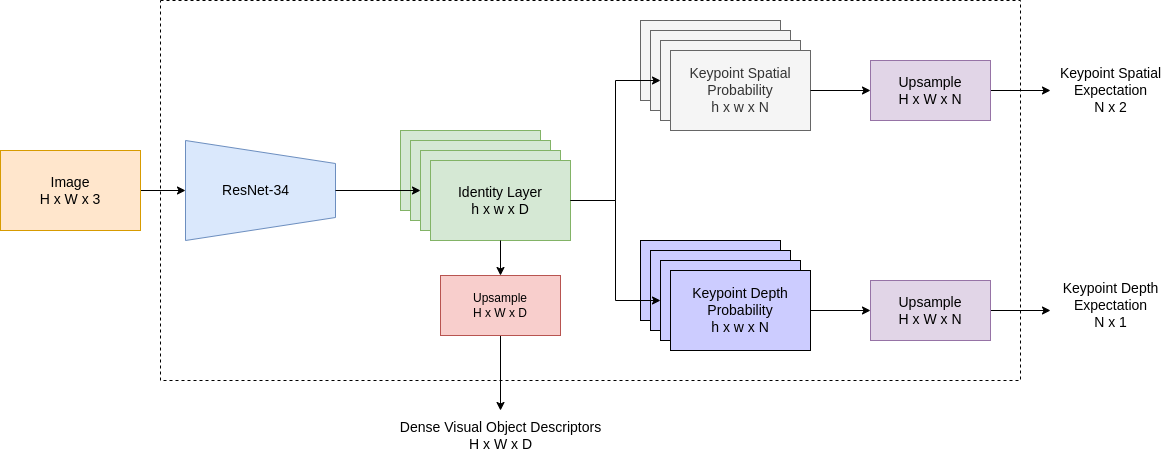
\includegraphics[scale=0.34]{images/arch.png}
    \caption{Illustration of the novel framework designed to compute and seamlessly extract dense visual object descriptors efficiently.
        During inference, we extract dense visual object descriptors directly from the network and ignore predicted spatial-depth expectations of the keypoints.}
    \label{fig:modified_dnn}
\end{figure}


\subsection{Loss Functions}

For training, we directly adopt silhoutte consistency loss ($\mathcal{L}_{obj}$), variance loss ($\mathcal{L}_{var}$) and separation loss ($\mathcal{L}_{sep}$) functions from \cite{suwajanakorn2018discovery} to train the network on the keypoint prediction task.
However, we modify the multi-view consistent loss and relative pose estimation loss. In the case of multi-view consistency loss we
project the predicted spatial-depth expectation using camera intrinsics as follows:
\begin{equation}
    X_{cam} \in \mathbb{R}^{3 \times 1} = \mathcal{I}_{cam}^{-1}  \ [u, v, 1.0]^T \times d \text{ , where  } \ \mathcal{I}_{cam} \in \mathbb{R}^{3 \times 3} \text{ and }  u, v, d \in \mathbb{R}^+.
\end{equation}

Furthermore, we project the camera coordinates of the keypoints from one camera viewpoint to another camera viewpoint using relative transformation supplied from the synthetic augmentation procedure as follows:

\begin{equation}
    \label{eqn:mvc}
    \mathcal{L}_{mvc} \in \mathbb{R} = \mathcal{H}(\hat{X}^B_{cam}, \mathcal{T}_{A \rightarrow B} \hat{X}^A_{cam}) \text{ , where  } \hat{X}_{cam}=[X_{cam}, 1.0]^T \in \mathbb{R}^{4 \times 1} ,
\end{equation}


In Equation~\ref{eqn:mvc}, $ \mathcal{T}_{A \rightarrow B} \in SE(3)$ is a Special Euclidean Group~\cite{thurston2014three} which
is relative transformation from camera-frame $A$ to camera-frame $B$. We use Huber loss $\mathcal{H}$ as it produces smoother gradients for framework optimization.
Furthermore, we do not discard the relative transformation information to calculate the relative pose loss as suggested in \cite{suwajanakorn2018discovery}.
Moreover, being influenced from \cite{zhao2020learning} we modified the relative pose loss as follows:
\begin{equation}
    \mathcal{L}_{pose} = \Vert log(\mathcal{T}_{truth}^{\dagger} \mathcal{T}_{pred}) \Vert \text{ , where  } \ log: SE(3) \rightarrow \mathfrak{se}(3) \text{ and } \mathcal{T}^{\dagger} = \begin{bmatrix}
        R^T & -R^T t \\
        0^T & 1
    \end{bmatrix}.
\end{equation}


\subsection{Robot Grasping Pipeline}
To use the proposed framework as a robot grasping pipeline, we extract dense visual object descriptors from the network and store
one single descriptor of objects in a database manually for now. During inference, we extract dense visual object descriptors from the network and
query the descriptor from the database to find the closest match as follows:
\begin{equation}
    \label{eqn:gaussian_kernel}
    \mathbb{E}{[u^*, v^*]_{d}} = \operatorname*{argmin}_{u, v} \ exp-\left(\dfrac{\|I_D[u, v] - d\|}{exp(t)}\right)^2 \text{ , where  } \|I_D[u, v] - d\| \in \mathbb{R}^{H \times W}.
\end{equation}
Where $t \in \mathbb{R}$ controls the kernel width influencing the search space to compute the optimal spatial expectation $\mathbb{E}{[u^*, v^*]_{d}}$ of
the query descriptor $d \in \mathbb{R}^D$ in the descriptor image $I_D \in \mathbb{R}^{H \times W \times D}$. The computed spatial expectation is projected to the robot frame using camera intrinsics and poses to perform a pinch grasp.
Furthermore, the Franka Emika 7-DOF robot manipulator with two jaw gripper and wrist-mounted Intel Realsense D435 camera is used as a testing setup as illustrated in Figure~\ref{fig:robot_setup}.

\begin{figure}[htb]
    \centering
    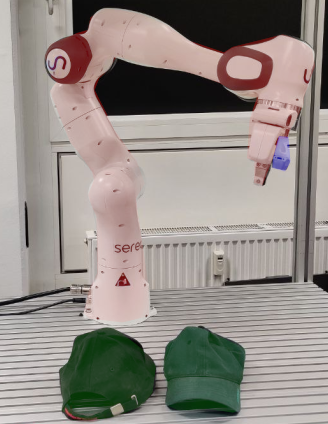
\includegraphics[scale=0.25]{images/franka.png}
    \caption{Illustration of the robot grasping pipeline setup. In the image, the robot is highlighted in red, the caps in green, and the camera in blue.}
    \label{fig:robot_setup}
\end{figure}